\documentclass[../Main.tex]{subfiles}

\begin{document}
\author{Photons} %use author for title of lesson
\date{Year 1 Topic 20} %use date to refer to topic in main booklet

\section{Photons} %Section is the title of the lesson repeated, ready for the main contents page.

\begin{frame}{Light as a wave}
     In the 1600s, Huygens presented the first evidence that light was a wave through refraction, dispersion, and reflection. And nobody disputed this, the evidence was enough and that was the end of that. 
     \pause
     \begin{figure}
         \centering
         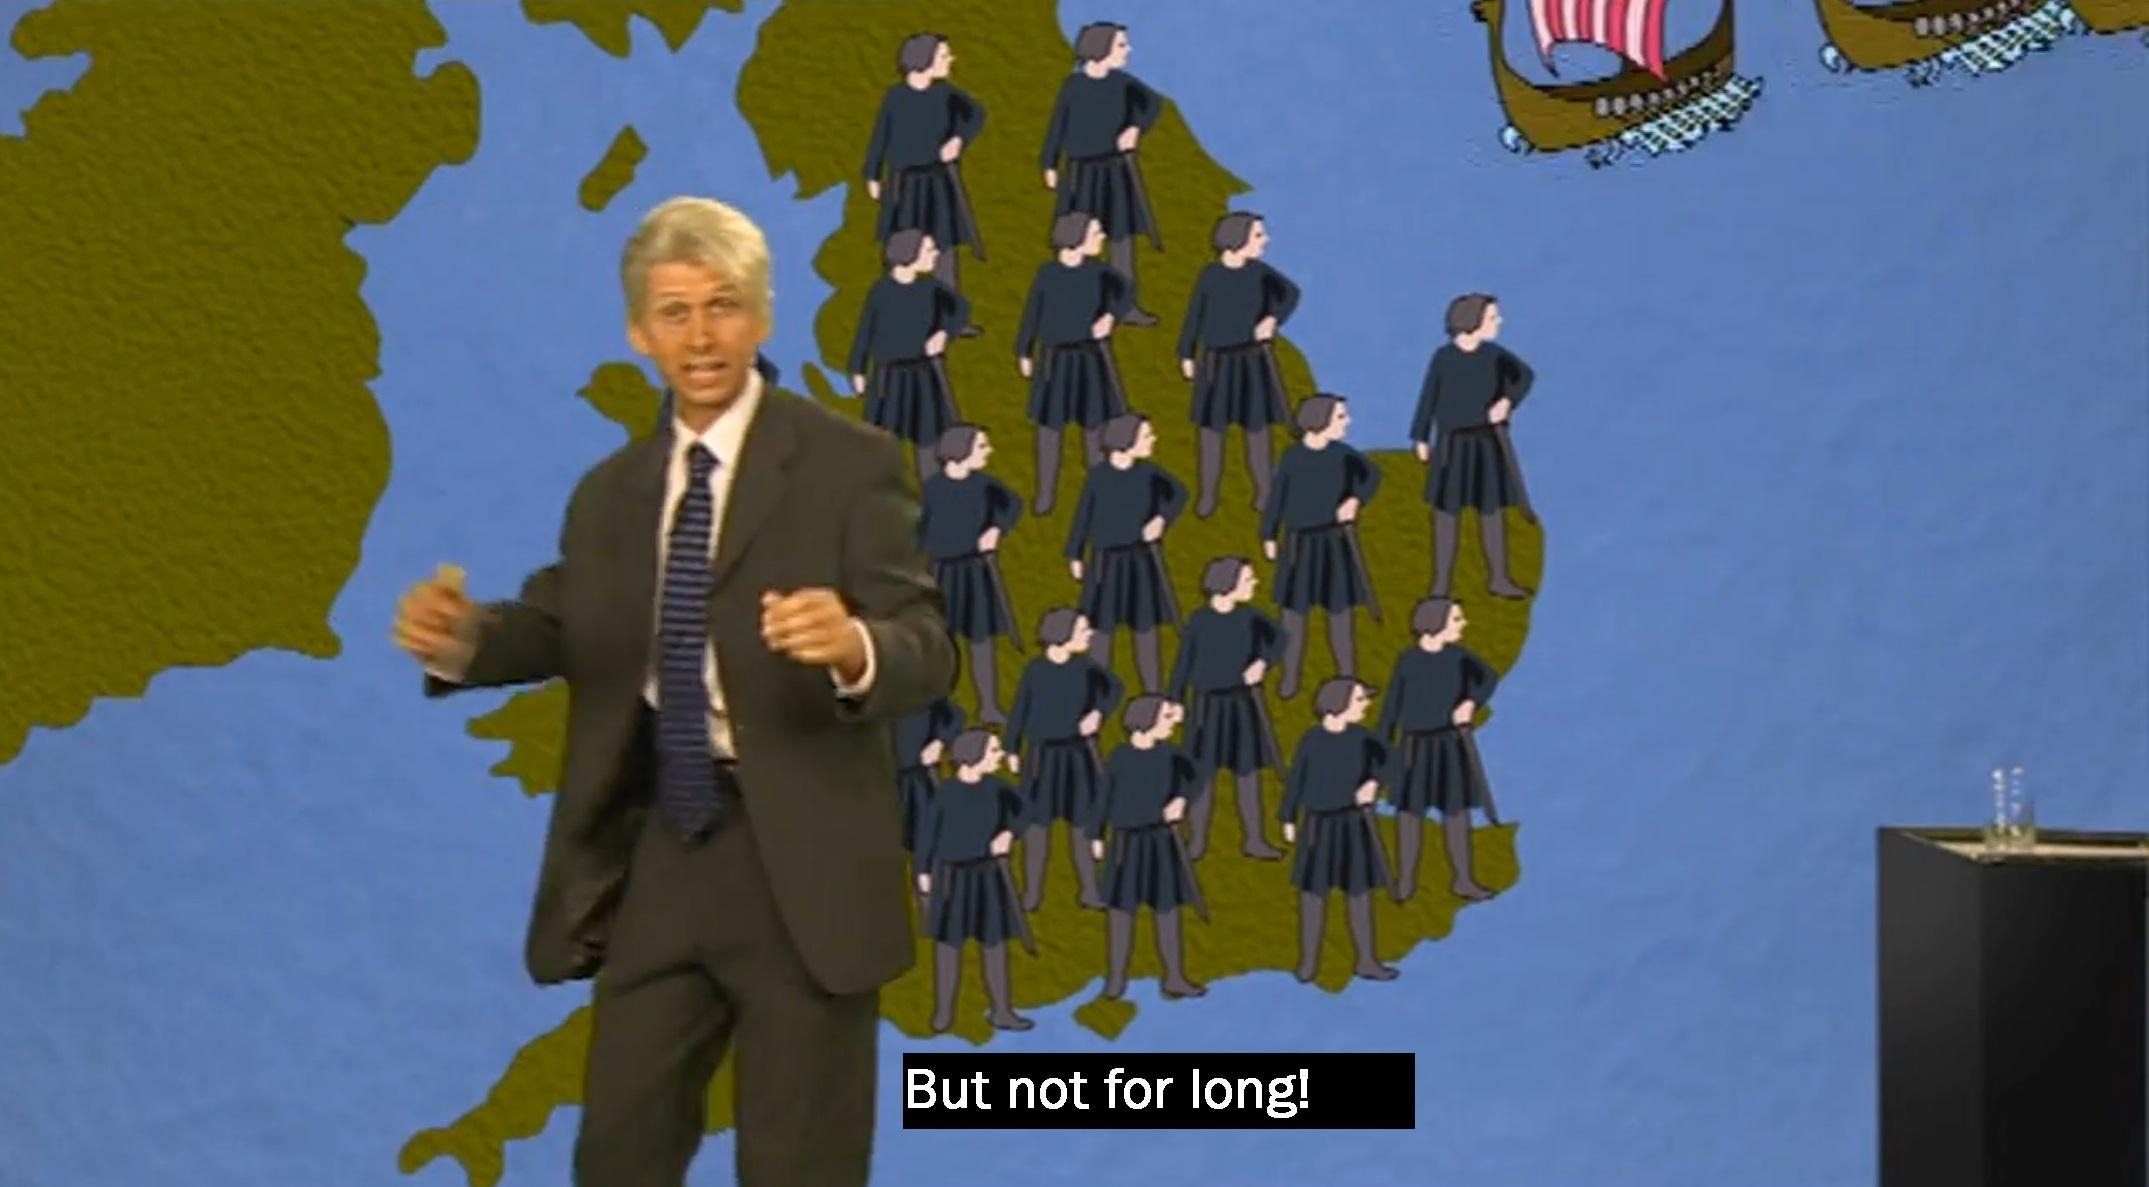
\includegraphics[height=3.5cm]{Quantum_Images/butnotforlong.jpg}
     \end{figure}
     Isaac Newton was already of high prestige due to his laws of motion, and posed an alternate hypothesis that light was a stream of particles known as corpuscles that moved at a finite speed - following along the ongoing hypothesis that matter was made of atoms that were indivisible.
\end{frame}

\begin{frame}{Competing theories}
    But because Newton's theory did not completely explain the behaviours of light known, his theory was abandoned and largely forgotten about and that was absolutely definitely the end of that.
    \pause
    \begin{figure}
        \centering
        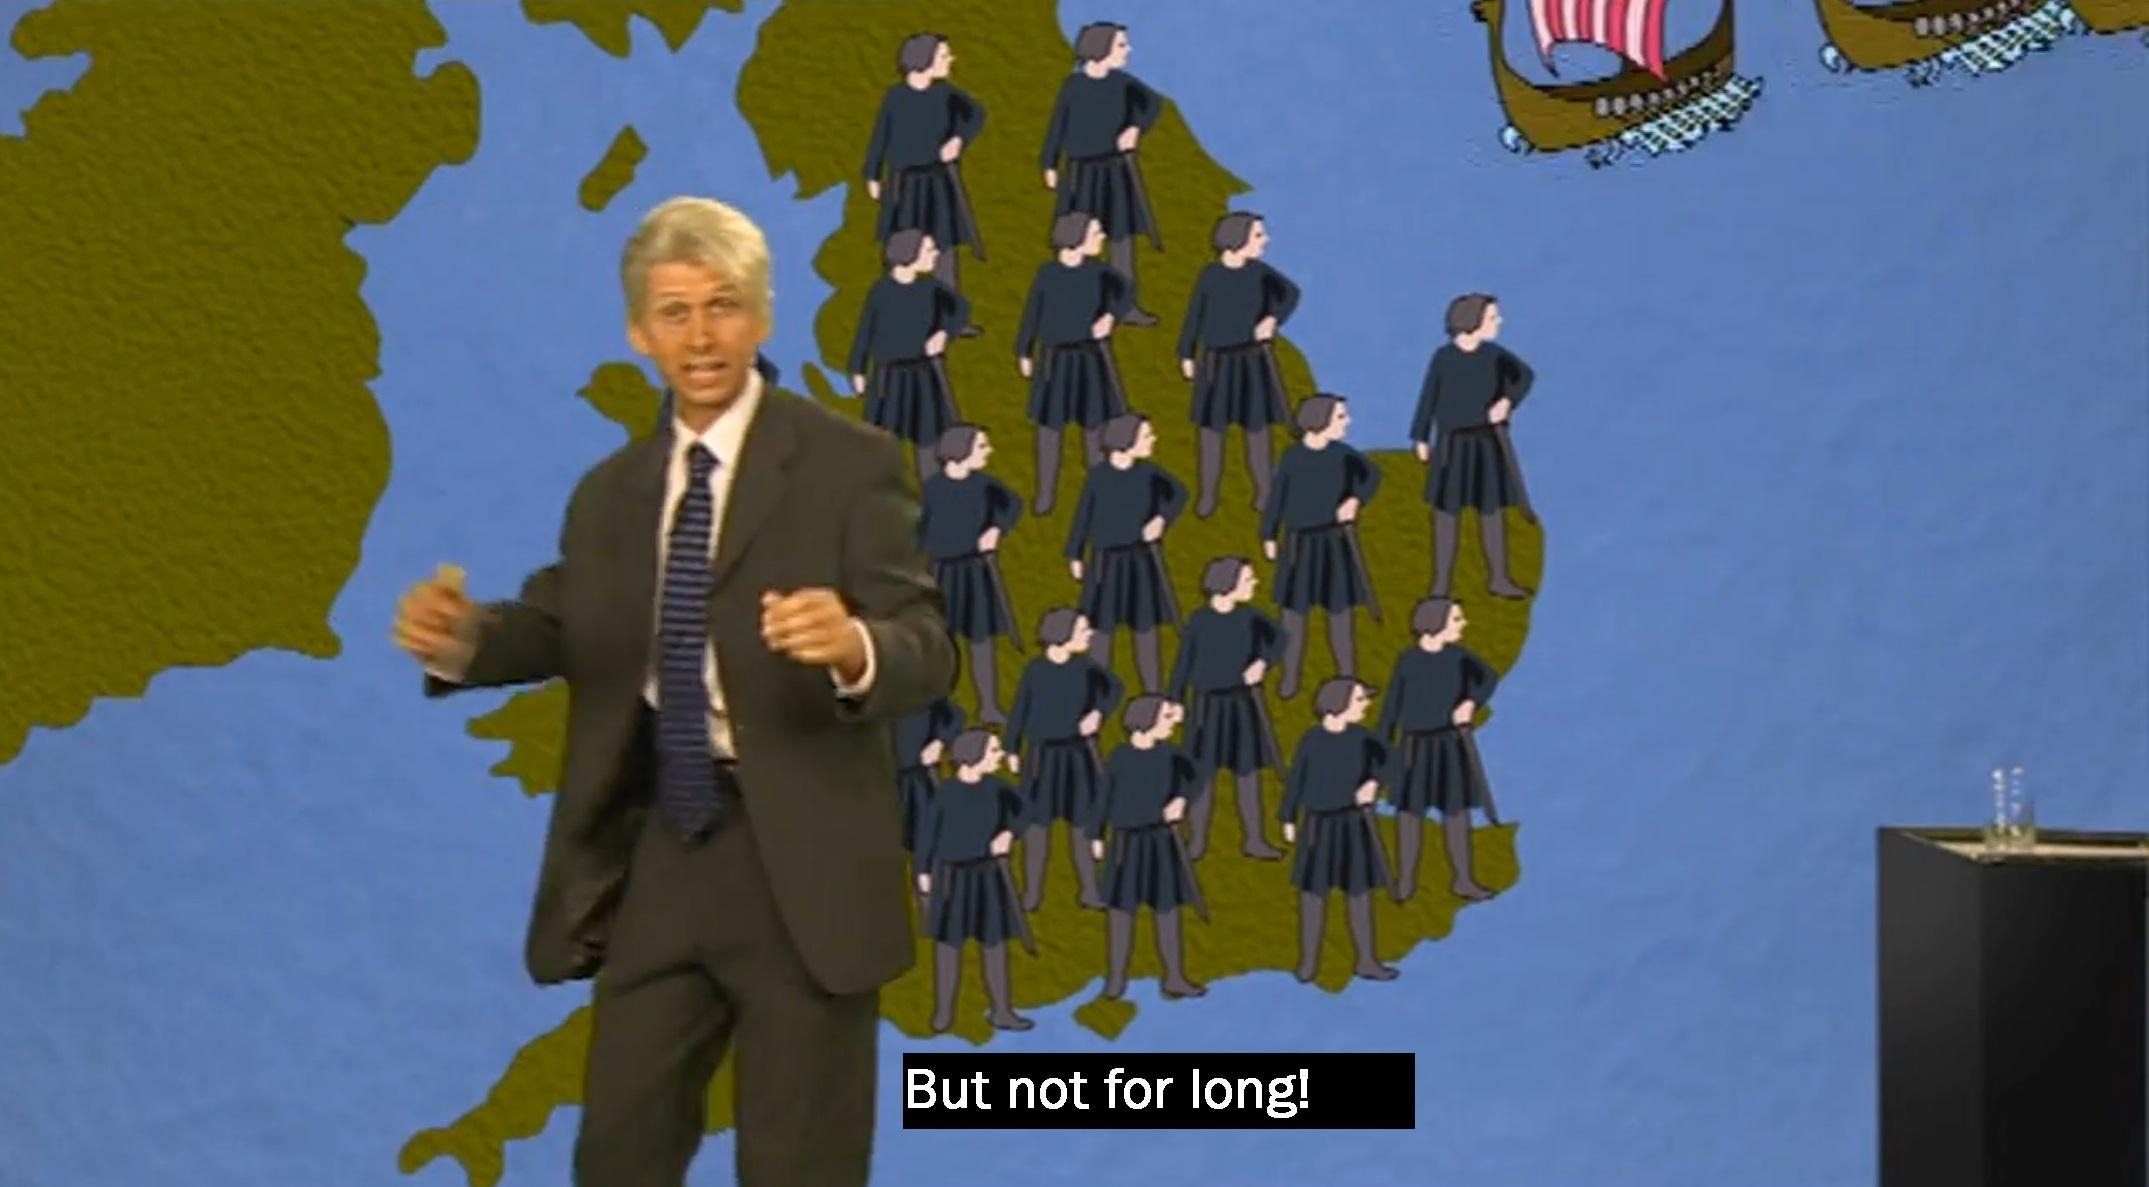
\includegraphics[height=3.5cm]{Quantum_Images/butnotforlong.jpg}
    \end{figure}
    In the early 20th century, new evidence came to light suggesting that light showed behaviours akin to that of a particle, whilst also showing behaviours of being a wave.
\end{frame}

\begin{frame}{Photons}
    This evidence we will discuss in further detail soon, but led to scientists calling these particles \emph{photons}, a similar naming convention to the electron, proton and neutron that were discovered in the 19th century.
    
    \begin{block}{Photon}
    A photon can be thought of as a packet of energy of quantised values -- meaning it can only take a certain value, hence the origin of \emph{quantum} physics. 
    \end{block} \pause
    
    The energy a photon can hold is given by 
    \begin{equation*}
        E=hf
    \end{equation*}
    where
    \begin{itemize}
        \item E is the energy of the photon in J
        \item f is the frequency of light (relating to the wave theory) in Hz
        \item and h being the \emph{Planck constant}, $h=6.63\times10^{-34}$Js, a value determined by Max Planck in the 20th century
    \end{itemize}
\end{frame}

\begin{frame}{Examples}
\begin{equation*}
    E=hf, \newline h=6.63\times10^{-34}Js
\end{equation*} (both given on your formula sheet)

    \begin{exampleblock}{Example 1}
    Ultraviolet radiation has a frequency of $6.8 \times 10^{15}$ Hz. Calculate the energy, in joules, of the photon. \pause
    --$4.5\times 10^{-18}$J.
    \end{exampleblock} \pause
    
    \begin{exampleblock}{Example 2}
    A ruby laser produces red light that has a wavelength of 500 nm. Calculate its energy in joules. \pause
    --$4\times 10^{-19}$J
    \end{exampleblock} \pause
    A shortcut method for if you do not have frequency but need energy (note that this is also given on your formula sheet):
    \begin{equation*}
        E=\frac{hc}{\lambda}
    \end{equation*}
\end{frame}

\begin{frame}{Energy of a photon}
    As can be seen, the energies involved are very very small. On the order of $10^{-19}J$. This can be difficult to work with, so we can introduce a new unit of energy, the electronvolt:
    
    \begin{block}{The electronvolt eV}
    $1eV = 1.6\times10^{-19}J$ and is equal to the kinetic energy of an electron that is accelerated through a potential of 1V (more on this with Electric Fields in 2nd year).
    \end{block}
    \pause
    \begin{exampleblock}{Examples}
    For the energies previously calculated, convert these into electronvolts. \pause
    -- 28eV, 2.5eV
    \end{exampleblock}\pause
    \begin{exampleblock}{Example 2}
    How many eV is 1J of energy? \pause
    --$6.3\times10^{18}eV$ -- or 6.3EeV
    \end{exampleblock}
\end{frame}

\begin{frame}{Energy of the EM Spectrum}
    List the EM spectrum, showing the direction of higher frequency, and shorter wavelength, but also now the direction of higher energy per photon. \pause
    \begin{figure}
        \centering
        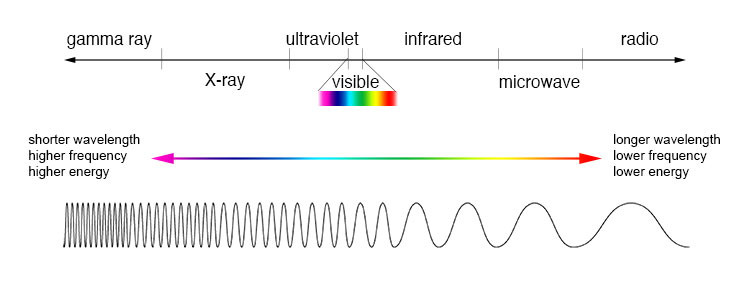
\includegraphics[width=\textwidth]{Quantum_Images/EM_spectrum_compare_level1_lg.jpg}
    \end{figure}
\end{frame}

\begin{frame}{Energy of the EM Spectrum}
    \begin{figure}
        \centering
        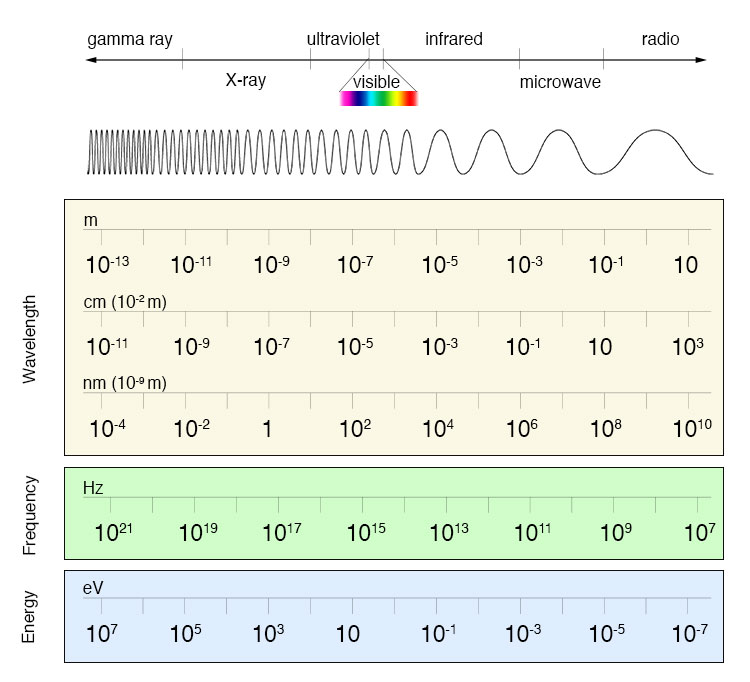
\includegraphics[height=7cm]{Quantum_Images/EM_spectrum_compare_level2_lg.jpg}
    \end{figure}
\end{frame}

\begin{frame}{Photons and LEDs}
    An LED will activate at a voltage of 0.7V, known as the threshold p.d. The energy transferred by an electron is the work done on the electron
    
    \begin{equation*}
        W=QV, = eV
    \end{equation*}
    This is approximately the energy emitted by a single photon of the LED
    \begin{equation*}
        eV = hf = \frac{hc}{\lambda}
    \end{equation*}
    This sets up an easy experiment to follow to determine the value of Planck's constant, where we can simply determine the threshold p.d of LEDs that emit a constant wavelength of light.
\end{frame}

\end{document}